% twocolumn を使うと2段組になる

%\documentclass[a4j,twocolumn]{jsarticle}        % -> platex
%\documentclass[a4j,twocolumn]{ujarticle}       % -> uplatex
\documentclass[uplatex]{jsarticle}   % -> uplatex + jsarticle

\usepackage{resume} % 他パッケージ,専用コマンド,余白の設定が書かれている

%%%%%%%%%%%%%%%%%%%%%%%%%%%%%%%%%%%%%%%%%%%%%%%%%%%%%%%%%%%%%%%%%%%%%%%%
% ヘッダ: イベント名,日付,所属,タイトル,氏名
%%%%%%%%%%%%%%%%%%%%%%%%%%%%%%%%%%%%%%%%%%%%%%%%%%%%%%%%%%%%%%%%%%%%%%%%

\pagestyle{plain}
\newcommand{\comment}[1]{}
\begin{document}
\twocolumn[
\beginheader{令和4年度 コンピュータサイエンス学部 輪講論文発表}{2022}{12}{22}{井上 研究室}
\title{弦楽合奏団の指揮体験にフィードバック機能を備えたVRコンテンツ}
\author{C0B20032 岡野 真士}
\endheader
]

\vspace{3mm}

 % 本番用ページ番号オフセット
\setcounter{page}{9}
%---------------------------------------------------------------------------
% 本文
%---------------------------------------------------------------------------


\section{はじめに}
オーケストラを指揮する指揮者は,一生に一度はやってみたい職業の一つと言われたこともある\cite{1}.

指揮者の主な役割は,楽器を演奏する演奏者のまとめ役となることであり,演奏者の表現力を高めることにある.
そして,指揮に必要な技術は曲のテンポを決めることであり,音の強弱などを指示することである\cite{2}.そこで,本研究では指揮の基本である曲の拍子やテンポを体験者が思い通りに刻み,それができているかどうかを確認できるコンテンツを提案する.体験者が指揮に没入して,様々なCG演出を活用できるようVR空間を利用した.
%参考文献[1]
%参考文献[4]
\footnote{弦楽合奏団の指揮体験にフィードバック機能を備えた VR コンテンツ 浅井 開 中沢 憲二
J-STAGE 日本バーチャルリアリティ学会論文誌2022年27巻3号235-244p
}
%---------------------------------------------------------------------------------------------
\section{関連研究}
数台のスマートフォンにオーケストラの演奏を奏でる楽 器を表示して演奏者と見立ててオーケストラを指揮する研究も報告された[10].
しかし,この方法ではオーケストラを目の前にしているという臨場感を得るのは難しい.

指揮の自己学習を目的として指揮の様子を自分自身で確認できるシステムに関する研究がある[16].しかし,右手の拍取りの識別をしていないため,4拍子で振れているかどうかの確認はできない.また,体験者に指揮動作の出来をリアルタイムでフィードバックするような機能も実装されていない.このように指揮者の学習支援に関しては,指揮の出来具合の検出方法や,検出結果の体験者へのフィードバック方法,そのフィードバックをもとに体験者がいかに修正していくかが課題である.

%参考文献[10]
%参考文献[16]
%------------------------------------------------------------------------------------------------
\section{制作したコンテンツ}
VR空間上に制作した弦楽合奏団を\figref{fig:gaikan}に示す.楽器アバタを使用して弦楽合奏団を表現した.

 \begin{figure}[b]
 \centering
 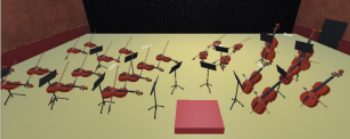
\includegraphics[clip,width=7cm]{gaikan.png}
 \caption{VR弦楽合奏団}\label{fig:gaikan}
\end{figure}
コンテンツの楽曲には,4拍子の曲を用いた.指揮の体験者は両手に持ったコントローラを操作し,音量,曲の再生速度をそれぞれ独立して制御するようにした.再生速度制御に必要なテンポは右手の指揮の動きから推定した.\figref{fig:hyousi}に4拍子の動きとそれを認識する仕 組みを示す.腕がI~IVの順に動いた場合に,4拍子が振れていると認識するようにした.テンポは,60秒を1拍の動作にかかった時間で除算して推定した.

4拍子を表現する腕の動きは,Y座標から検出した1拍の動作に着目し,1拍の間にコントローラが左に移動した場合を1,右に移動した場合を2とし,それを順に記録していく.その並び方が,あらかじめ設定した4拍子のパターンに1つでも該当すれば4拍子ができていると判定した.

 \begin{figure}[b]
 \centering
 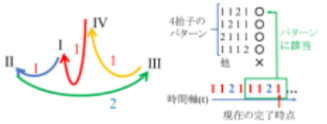
\includegraphics[clip,width=7cm]{hyousi.png}
 \caption{4拍子の動作判定の仕組み}\label{fig:hyousi}
\end{figure}
 
実験では,4拍子の成功や失敗にかかわらず,最後まで演奏を再生するようにした. 

体験者が装着したHMD(Head Mounted Display)を通して観察するコンテンツのシーンを\figref{fig:sikumi}に示す.

 \begin{figure}[b]
 \centering
 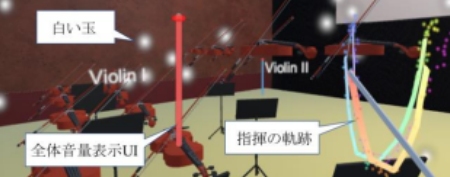
\includegraphics[clip,width=7cm]{sikumi.png}
 \caption{指揮を体験している様子}\label{fig:sikumi}
\end{figure}

また,指揮の成功回数の積み重ねとして示す累積回数に応じて,軌跡の色が「赤→黄→緑→青→紫→ 虹」と変化する.その規則を\figref{fig:sikumi}に示す.

\begin{figure}[t]
 \centering
 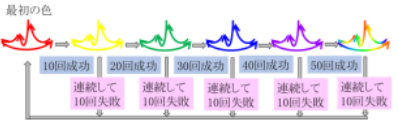
\includegraphics[clip,width=7cm]{sikisikumi.png}
 \caption{指揮軌跡の色の変化の規則}\label{fig:hoge}
\end{figure}

%--------------------------------------------------------------

\section{実験}
\subsection{実験方法}
この実験を行う前に予備実験を行った.その結果に基づき,以下4つの点を修正した.
\begin{enumerate}
\item 指揮指標UIの表示
\item 軌跡の色の変更,4拍子失敗時に赤色かつ波線に変更
\item 4拍子失敗の判定を10回から7回へ変更
\item 4拍子失敗時に曲を変調
\end{enumerate}

\figref{fig:UI}に指揮指標UI,\figref{fig:henka}に指揮軌跡の色の変化を示す.

\begin{figure}[b]
 \centering
 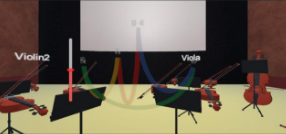
\includegraphics[clip,width=7cm]{sikiUI.png}
 \caption{指揮指標UI}\label{fig:UI}
\end{figure}

\begin{figure}[b]
 \centering
 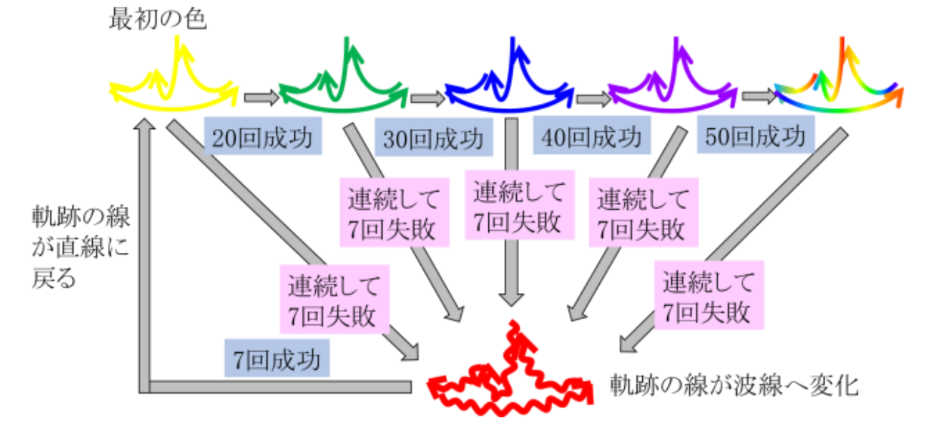
\includegraphics[clip,width=7cm]{kisekihenka.png}
 \caption{指揮軌跡の色の変化}\label{fig:henka}
\end{figure}

改善したコンテンツを用いて,指揮指標UIと4拍子失敗時の視聴覚演出の効果検証を目的に実験を実施した.被験者は大学生予備実験と同じ大学生12 名とした.コンテンツの体験後,アンケート調査を実施した.

%------------------------------------------------------------------------------

\subsection{実験結果}
4拍子の指揮をする際に指標UIが効果的に作用したかどうかについてアンケート調査を行った.その結果,被験者全員から役立ったとの回答が得られ,指標UIの表示は有効であることが分かった. 

また,4拍子失敗時の気づきについて記録たデータを分析し定量的に調べた.結果は\figref{fig:miss}に示す通りである.

\begin{figure}[t]
 \centering
 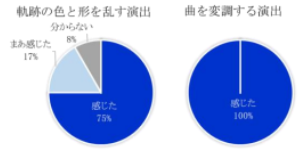
\includegraphics[clip,width=7cm]{miss.png}
 \caption{4拍子失敗時の視覚的演出への気づきの結果}\label{fig:miss}
\end{figure}

\section{まとめ}
指揮の基本である曲の拍子やテンポを思い通りに刻 め、それをVR空間で確認できるコンテンツを開発した。指揮者としての楽しさや 難しさを、さらに味わってもらうためには、本コンテンツ は一側面にすぎないため、多方面からの検討が必要と 考える。 
今回のように演奏という「音」に関わるコン テンツでは、視覚的な演出よりも聴覚的な演出の効果 が高く、音の変化に対して被験者は敏感になっていたと 考えられる。

身体の動きをと もなう体験型 VR コンテンツおいて、視覚のみならず聴 覚等他の感覚を使って体験状況を適切にフィードバッ クすることで、体験者をよりコンテンツに引き込める可能 性がある。 
%---------------------------------------------------------------------------
% 本文終わり
%---------------------------------------------------------------------------

 % 参考文献
\begin{thebibliography}{9}
 \bibitem{1}  椿音楽教室, “指揮者の役割とは?なるにはどうすれば いい?”: 
https://tsubaki-musicschool.com/blog/useful-column/2193 6/
\bibitem{2} 岡部洋一, 指揮法:  
http://www.moge.org/okabe/temp/conduct.pdf 
\bibitem{3} Chun Kit TsUI, Chi Hei Law, Hongbo Fu: One-Man  Orchestra: Conducting Smartphone Orchestra; The City  University of Hong Kong, (2014) 
\bibitem{4} 佐野文哉, 藤原克哉, 斎藤正親, 四反田素幸, 水戸部 一季: VR 空間における指揮動作の学習支援技術の研 究; 第 23 回日本バーチャルリアリティ学会大会論文集, (2018) 
\end{thebibliography}

\end{document}


%-----------------------------------------------------
% テンプレート
%------------------------------------------------------------------------------

%-----------
%% 箇条書き
%-----------
%\begin{itemize}
% \item
%\end{itemize}

%-------------------
%% 番号付き箇条書き
%-------------------
%\begin{enumerate}
% \item
%\end{enumerate}

%-----------
%% 図の表示
%-----------
%\begin{figure}[H]
% \centering
% \includegraphics[clip,width=7cm]{hoge.eps}
% \caption{図タイトル}\label{fig:hoge}
%\end{figure}

%-----------
%% 図の参照
%-----------
%\figref{fig:hoge}

%-----------
%% 表の作成
%-----------
%\begin{table}[H]
% \centering
% \caption{表タイトル}\label{tab:fuga}
% \begin{tabular}{|c|c|c|}\hline
%  hemo & piyo & fuga \\ \hline
%  hemo & piyo & fuga \\ \hline
% \end{tabular}
%\end{table}

%-----------
%% 表の参照
%-----------
%\tabref{tab:fuga}

%-----------
%% 参考文献
%-----------
%\begin{thebibliography}{9}
% \bibitem{piyo} 参考文献
%\end{thebibliography}

%-----------------
%% 参考文献の参照
%-----------------
%\cite{piyo}
